\documentclass[11pt]{article}

\usepackage{helvet}
\renewcommand{\familydefault}{\sfdefault}

\usepackage{amsmath,amssymb,amsthm}
\usepackage{graphicx}
\usepackage{subfigure}
\usepackage{caption}
\usepackage{mathtools}

\usepackage[top=1in,bottom=1in,left=1in,right=1in]{geometry}
\usepackage{paralist}

\usepackage[pagebackref=true,colorlinks=true,breaklinks=true,linkcolor=blue,citecolor=blue,urlcolor=blue]{hyperref}

\usepackage{fancyhdr}
\setlength{\headheight}{15.2pt}
\pagestyle{fancyplain}
\lhead[RUI]{RUI} 
\chead[hTeXML: Web Authoring for STEM]{Web Authoring for STEM}
\rhead[C. Aguilar]{C. Aguilar}

% Move sections heading to the center
\usepackage[center]{titlesec}
\titleformat{\section}[hang]{\normalfont\scshape}{\thesection.}{.5em}{\filcenter}[]
\titleformat{\subsection}[hang]{\normalfont\scshape}{\thesubsection.}{.5em}{\filcenter}[]

% Changes title of bibliography
\renewcommand\refname{\textbf{\Large References}}

% Theorem environments
\newtheoremstyle{theorem}{3pt}{3pt}{\itshape}{}{\bfseries}{.}{.5em}{}
\theoremstyle{theorem}
\newtheorem{theorem}{Theorem}
\newtheoremstyle{definition}{3pt}{3pt}{\normalfont}{}{\bfseries}{.}{.5em}{}
\theoremstyle{definition}
\newtheorem{definition}{Definition}

% Spacing commands
%\usepackage{bibspacing}
%\setlength{\bibspacing}{6pt}

% User defined commands


%=========================================================
\begin{document}

\begin{center}
\textbf{\Large Project Description}\\[0.25cm]
\hrulefill\\[0.5cm]
\textbf{\Large Facilitating the Creation of Open-Access Educational \\[0.25cm] STEM Resources for Improved Student Learning and Engagement}\\
\hrulefill
\end{center}
\baselineskip 1.5em

%=========================================================
\section{Introduction: OER Resources}


\subsection{Cost of College Textbooks: Relief on the Horizon?}
Students, parents, and educators are well aware of the exorbitant prices for some college textbooks.  Using data from the Bureau of Labor Statistics, economist Mark J. Perry of the University of Michigan\textendash Flint published a chart in 2018 that shows the price changes of several goods and services from 1997 to 2018 \cite{perry2018}.  The chart shows that the price of textbooks increased by 204\% from 1997-2018.  The chart is updated every 6 months and the latest update was published in July 2022 \cite{perry2022}; see Figures~\ref{fig:cpi-textbooks-2018}-\ref{fig:cpi-textbooks-2022}.  Based on the data, college textbook prices have increased between 5-6\% annually on average which is well above the average annual inflation rate of 2\% over the same period.  Interestingly, Perry points out that beginning in 2017 and up to 2020, the price of college textbooks saw flat and small declines, with 2021 experiencing a small increase of 1.4\%.  Perry writes that the ``\textit{two consecutive annual decreases in 2019 and 2020 and the small increase in 2021 have been an unprecedented departure from a half-century of increases in educational book prices that averaged more than 6\% between 1968 and 2018}''.  Perry goes on to say that the price changes in textbooks could be attributed to the competition faced by traditional publishers from ``open textbooks'' and cites as examples the \href{https://open.umn.edu/opentextbooks}{Open Textbooks Library} and \href{https://openstax.org/}{OpenStax} websites as sources of hundreds of textbooks available for free.

\begin{figure}[h!]
\begin{minipage}[t]{8.0cm}
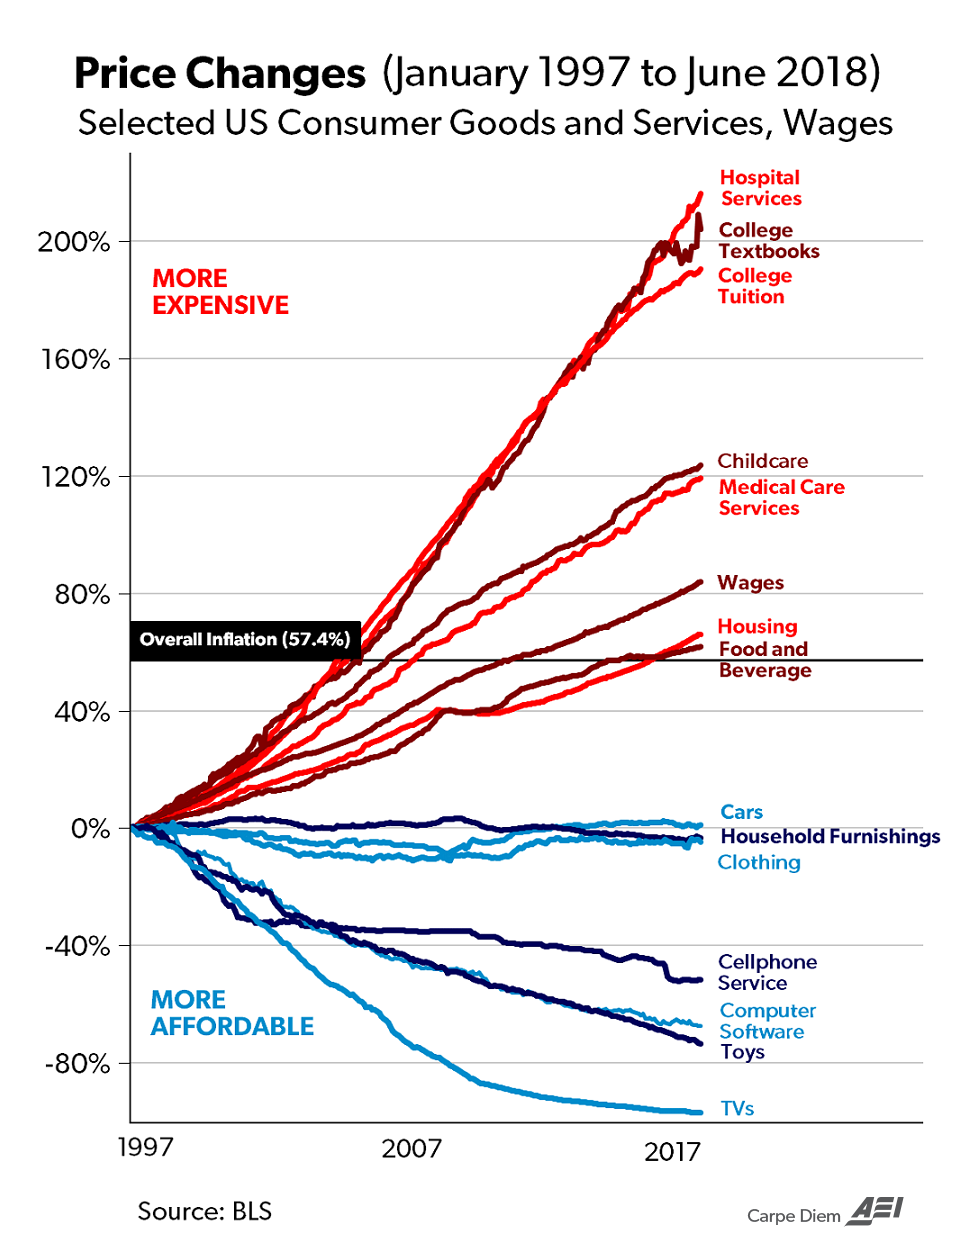
\includegraphics[width=70mm,height=80mm]{cpichart2018a.png}
\caption{\small From January 1997 to June 2018, the price of college textbooks has increased by approximately 204\%. (source: \href{aei.org/carpe-diem}{aei.org/carpe-diem}) }\label{fig:cpi-textbooks-2018}
\end{minipage}
\hfill
\begin{minipage}[t]{8.0cm}
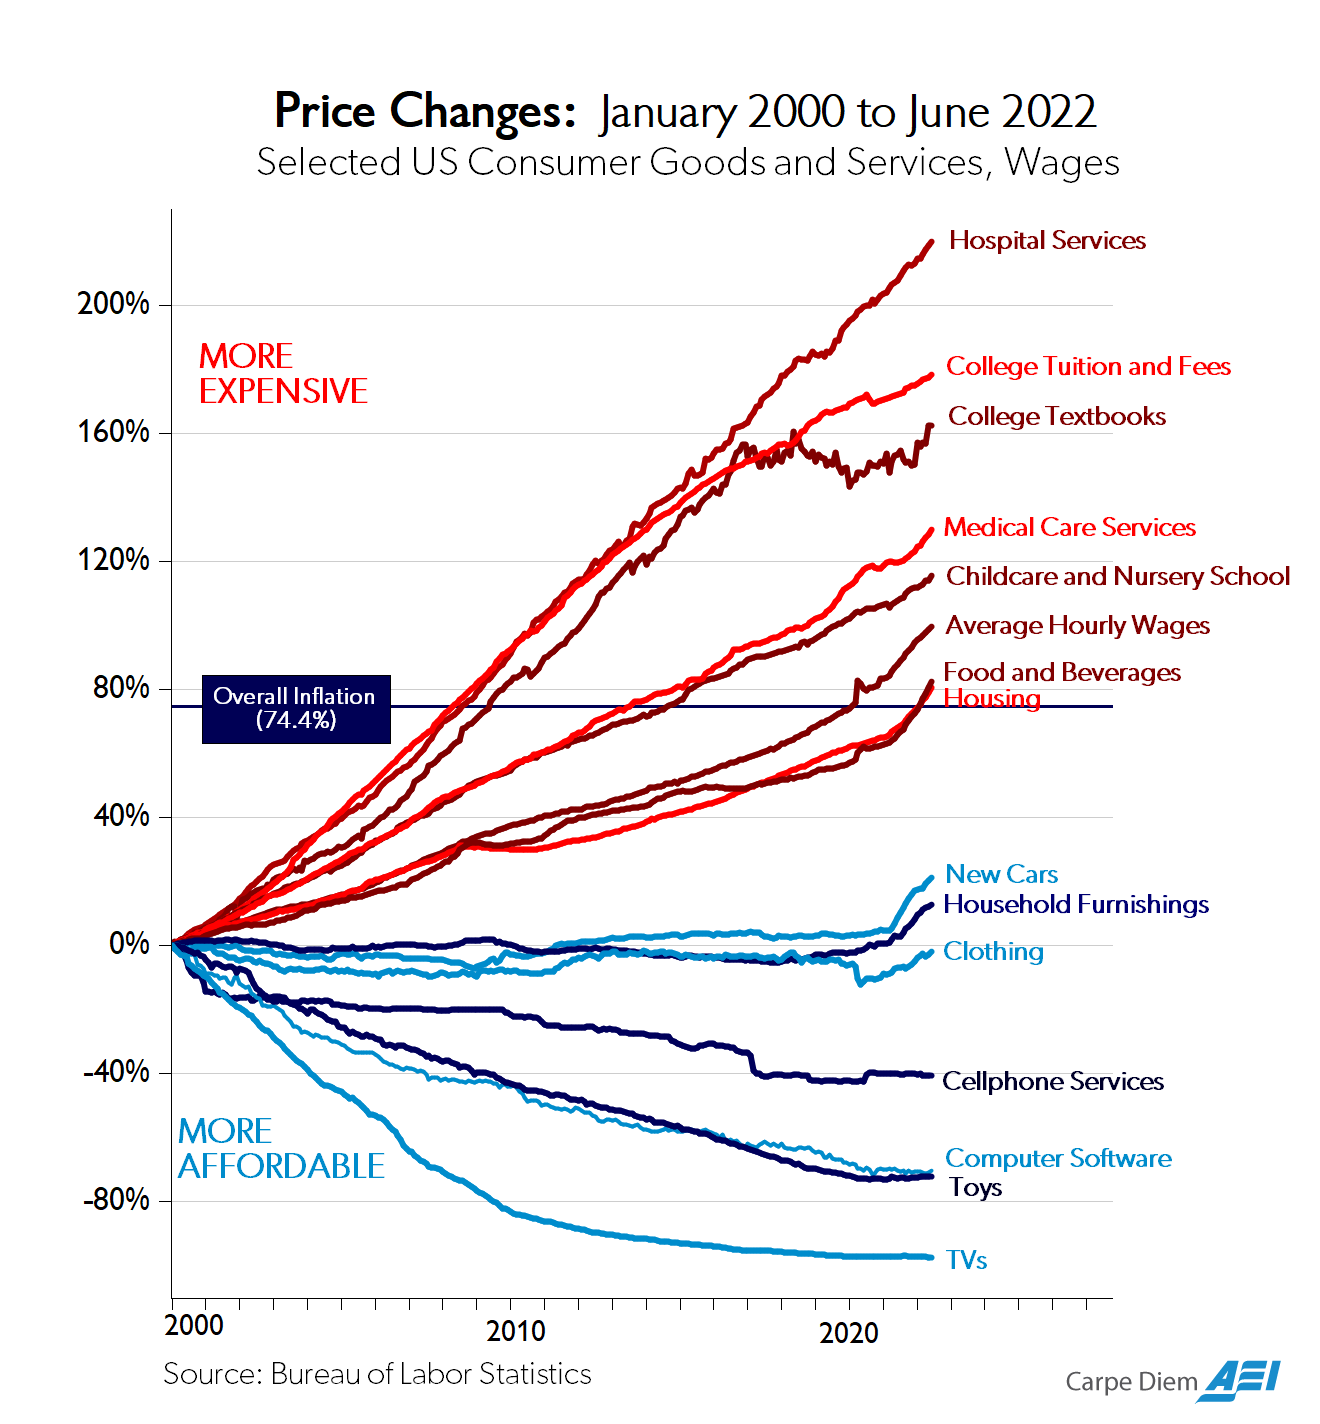
\includegraphics[width=70mm,height=82mm]{cpi2022junea-3.png}
\caption{\small From January 2000 to June 2022, the price of college textbooks has increased by approximately 162\%. (source: \href{aei.org/carpe-diem}{aei.org/carpe-diem})}\label{fig:cpi-textbooks-2022}
\end{minipage}

\end{figure}



%=========================================================
\section{Project Proposal}



\subsection{Overview}

%=========================================================
\subsection{Existing Technology}

\subsubsection{MathML}
\textbf{Mathematical Markup Language} (MathML) is a language used to describe the presentation and content of mathematical notation.  MathML is used in web browsers, in computer algebra systems (CAS), print typesetting, and voice synthesis.  The goal of MathML is to enable mathematically rich documents on the web in the same way that HTML has enabled this functionality for text; MathML markup can be written alongside HTML markup.  MathML markup can become quite complicated even for simple mathematical expressions.  As an example, the MathML markup to describe the mathematical expression
\[
x = \frac{-b \pm\sqrt{b^2-4ac}}{2a}
\]
is given by
\begin{verbatim}
    <math>
      <mi>x</mi><mo>=</mo>
      <mfrac>
        <mrow>
          <mo>-</mo><mi>b</mi><mo>&pm;</mo>
          <msqrt>
            <msup><mi>b</mi><mn>2</mn></msup>
            <mo>-</mo><mn>4</mn><mi>a</mi><mi>c</mi>
          </msqrt>
        </mrow>
        <mrow><mn>2</mn><mi>a</mi></mrow>
      </mfrac>
    </math>
\end{verbatim}
whereas the equivalent LaTeX markup is
\begin{verbatim}
    \[
        x = \frac{-b \pm \sqrt{b^2-4ac}}{2a}
    \]
\end{verbatim}
Needless to say, typing MathML by hand can be very tedious and error prone and as such it is not intended to be edited by hand.  Instead, the generation of MathML markup is usually the task of specialized equation editors or the result of a conversion from another markup language such as LaTeX.
 
\subsubsection{LaTeX2HTML}
\textbf{LaTeX2HTML} is a command line utility that converts LaTeX documents to web pages in HTML (latex2html.org).  As described on the programs website, ``\textit{LaTeX2HTML replicates the basic structure of a LaTeX document as a set of interconnected HTML files which can be explored using automatically generated navigation panels. The cross-references, citations, footnotes, the table of contents and the lists of figures and tables, are also translated into hypertext links. Formatting information which has equivalent tags in HTML (lists, quotes, paragraph breaks, type styles, etc.) is also converted appropriately. The remaining heavily formatted items such as mathematical equations, pictures or tables are converted to images which are placed automatically at the correct positions in the final HTML document''.}\footnote{latex2html.org}  Although LaTeX2HTML's goal of converting LaTeX documents to web pages is similar in spirit to htexml, there are core design features that distinguish LaTeX2HTML and htexml, such as:

\begin{itemize}
\item Documentation for LaTeX2HTML is scarce and not easily accessible for an average computer user.  Basic usage of LaTeX2HTML is not available on the projects website or github page.
\item LaTeX2HTML's conversion of mathematical equations to images to be rendered by the browser is in conflict with the goal of creating mathematically rich documents on the web that are rendered natively by the browser.
\item LaTeX2HTML is written in \textbf{perl} and must be installed from source using using configure, make, and make install or is available as a package for Linux or through the MacOS package manager Homebrew.
\item After installation, the program is available as a command line utility whereas all the functionality of htexml is accessible from a browser.
\item Even for an experienced computer user, installing LaTeX2HTML from source or via Homebrew can present its challenges that could discourage users from using the program.  htexml requires no installation.
\end{itemize}

\subsubsection{TeX4ht}
\textbf{TeX4ht} is a command line tool that converts LaTeX documents to various output formats including HTML, ODT (open document format), or DocBook.  According to the programs documentation, modern TeX distributions such as TeX Live and Miktex come with TeX4ht and a related bundling tool called \textbf{make4ht}.  



%=========================================================
\subsection{Placeholder}


%=========================================================
\section{Research Plan and Timeline}


\noindent\textbf{First Year:}  

\noindent\textbf{Second Year:}  

\noindent\textbf{Third Year:}  
%=============================================
\section{Broader Impacts}

\subsection{Research Impact}


%=============================================
\subsection{Training of STEM Students}

\subsection{Educational Impact}    


%=============================================
\newpage

% Bibliography
\begin{thebibliography}{99}
  \bibitem{perry2018} Mark J. Perry, {\em The CD `chart of the Century' Makes the Rounds at the Federal Reserve}, Carpe Diem (July 13, 2018), \href{https://www.aei.org/carpe-diem/the-chart-of-the-century-makes-the-rounds-at-the-federal-reserve/}{https://www.aei.org/carpe-diem/the-chart-of-the-century-makes-the-rounds-at-the-federal-reserve/}.

  \bibitem{perry2022} Mark J. Perry, {\em Chart of the Day \ldots or Century?}, Carpe Diem (July 23, 2022), \href{https://www.aei.org/carpe-diem/chart-of-the-day-or-century-8/}{https://www.aei.org/carpe-diem/chart-of-the-day-or-century-8/}
\end{thebibliography}


\end{document}
